%===================================== CHAP 3 =================================

%\chapter{Method}
\chapter{Conceptual design}
%\chapter{Approach and methodology}

\section{Overall Approach}

%%forklare hva jeg prøver å gjøre på en generell måte. introdusere pipelinen
Wikipedia is a web page presenting articles for the user. This leads to high focus on the usability related to users searching and reading articles. Because of this one can say that their articles are stored as an atomic entity in their database. An articles has no internal structure, except for the markup used to present it. That means that a process is needed to identify and extract examples from Wikipedia articles. This 
project%%Hva burde jeg kalle dette?
looks into the pipeline technique for this process. As explained in section \ref{pipeline}, a pipeline consist of multiple independent processes loosely coupled.\\


%\section{Prerequisite knowledge}

\section{Pipeline}

Write something about the approach being for data mining. Where to different methods where explored. Focus on how it was done.

\subsection{Existing pipeline} \label{smila}

In the early stages of the project, an existing project called SMILA was explored. SMILA crawls the web to extract information and then stores the information in an index. It has a REST API to control the system and for searching the index. The SMILA architecture is also based on the pipeline architecture containing the following processes jobs, crawling, storage, indexing and querying. With SMILA being very complex, it gains asynchronicity as its biggest benefit from the pipeline architecture. The SMILA pipeline also allows custom made pipelets to be inserted into the pipeline. A pipelet is a sub process inside a pipeline. By creating pipelets, the behaviour of SMILA could be tailored into extracting the relevant information from Wikipedia.

By only writing pipelets and then make SMILA use them when crawling Wikipedia, the project could concentrate the effort on identifying and indexing the examples. Unfortunately SMILA is an old and complex system, and is rarely updated anymore. When problems running SMILA appeared, it was quite troublesome to understand why and fix the issue. This ironically lead to all the effort in the starting phase being used on making SMILA run properly, instead of looking into the characteristics of examples. 

\begin{figure}[h]
\caption{An overall overview of the SMILA architecture}
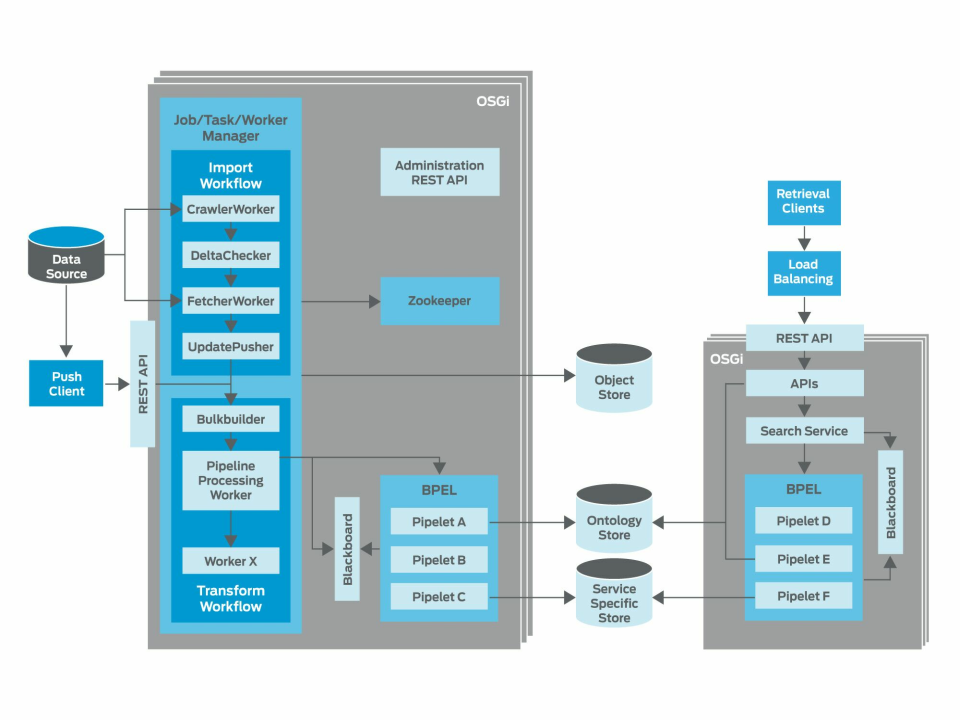
\includegraphics[width=\textwidth]{SMILA_Architecture}
\end{figure}

\subsection{Creating myself}

As described in section \ref{smila}, SMILA did not end up being a helpful tool for this project.

\begin{figure}[h]
\caption{A conceptual overview of the pipeline used to extract and index examples}
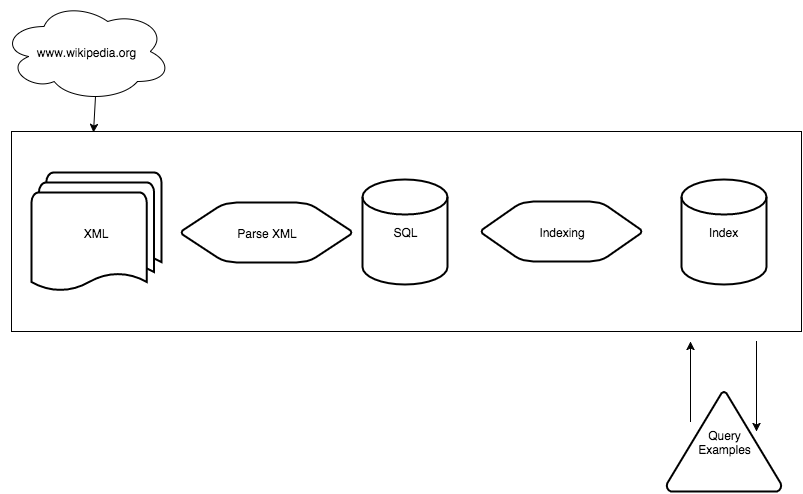
\includegraphics[width=\textwidth]{PipelineConcept}
\end{figure}


XML Parsing

\section{Database}

\section{Analysis of examples}
strucutre/characteristics of an example\\
what is good and bad example

\cleardoublepage